% BEGIN TEMPLATE
\documentclass{article}
\usepackage{graphicx}
\usepackage{hyperref} 
\usepackage{xcolor}
\usepackage{nameref}
\usepackage{listings}
\usepackage{float}
\usepackage[title]{appendix}
\graphicspath{ {../../images/} }
% CHANGE THESE
\newcommand{\courseListing}{CSCI 8110-001}
\newcommand{\courseName}{Advanced Machine Learning Applications}
\newcommand{\assignmentTitle}{Homework Assignment \#2}
\newcommand{\assignmentSubtitle}{Explainable Machine Learning}
\usepackage{geometry}
\geometry{margin=1in}

\hypersetup{
    colorlinks,
    linkcolor={red!50!black},
    citecolor={blue!50!black},
    urlcolor={blue!80!black}
}
\urlstyle{same}
\definecolor{codegreen}{rgb}{0,0.6,0}
\definecolor{codegray}{rgb}{0.5,0.5,0.5}
\definecolor{codepurple}{rgb}{0.58,0,0.82}
\lstdefinestyle{mystyle}{
    commentstyle=\color{codegreen},
    keywordstyle=\color{magenta},
    numberstyle=\tiny\color{codegray},
    stringstyle=\color{codepurple},
    basicstyle=\ttfamily\footnotesize,
    breakatwhitespace=false,         
    breaklines=true,                 
    captionpos=b,                    
    keepspaces=true,                 
    numbers=left,                    
    numbersep=5pt,                  
    showspaces=false,                
    showstringspaces=false,
    showtabs=false,                  
    tabsize=2
}

\lstset{style=mystyle}

\begin{document}
  \begin{center}
  
\includegraphics[scale=0.15]{UNO-Logo-Color.png}
  \\[0.3in]
  \textbf{\courseListing{}}\\
  \courseName{}
  \\[0.75in]
  \textbf{\assignmentTitle{}}\\
  \assignmentSubtitle{}
  \\[0.75in]
  \textbf{Patrick Davlin}
  \\[0.75in]
  \textbf{Computer Science Department}\\
  \textbf{Peter Kiewit Institute}\\
  \textbf{University of Nebraska}
  \\[0.75in]
  \textbf{Fall 2020}
  \\[0.3in]
  
\includegraphics[scale=0.075]{UNO-Icon-Color.png}
  \newpage
\end{center}
  \graphicspath{{./images/}}
% END TEMPLATE

\section{Project Setup}
\par Similar to the prior assignment, all work in this project was developed and executed using the Paperspace Gradient service.
Gradient allows for rapid setup of TensorFlow notebooks on GPU-powered machines.
A static version of the notebook can be accessed by clicking on \href{https://console.paperspace.com/te7vzjiu3/notebook/pr4zcy28o}{this link}.
\par Moreover, per the provided instructions, the Keras Vis library was used to simplify the process of implementing the concepts discussed in class.
There are many effective libraries built on top of the Keras toolset for this kind of application, allowing for very direct implementation and understanding of the processes used to visualize model outputs.
Several of the key features of this library will be discussed in the \nameref{impl} section.

\section{Process \& Results}
\subsection{Method Selection}
In approaching this project, the first step was to try and gain more familiarity on the concepts of saliency mapping and class activation maps (CAMs, specifically implemented in the course material via Grad-CAM).
There is a good deal of academic literature around both approaches available on the internet for comparison.
Ultimately, the decision of which to implement for this project (only one being required) was arbitrary; the CAM approach was chosen primarily because of the more vibrant colors of its output in documentation online.
While not a terrifically academic method by which to select a project, it was ultimately somewhat of a coin flip to decide what to implement.

\par To start, a few papers on CAMs were consulted. One in particular, by Selvaraju et al., helped to explain how Grad-CAM works, by finding gradients that associate features in some given image with their importance to a pre-selected target class \cite{Selvaraju2020}.
The final gradient can then be laid over the original image to \textit{explain} how the model arrived at its conclusion.

\subsection{Implementation} \label{impl}
\par The Keras Vis library linked in the assignment is not compatible with Tensorflow 2.0, which was used for the previous assignment and this one.
With that in mind, the \lstinline{tf-keras-vis} library was used from \href{https://github.com/keisen/tf-keras-vis}{GitHub} instead.
It was similarly straightforward as the Keras Vis documentation, allowing for relatively quick implementation of Grad-CAM for the purpose of visualizing the concept.
\par To start, an image is loaded from the filesystem, and the top five predictions are obtained from Keras' VGG16 model, as follows:

\begin{lstlisting}[language=Python]
img1 = load_img('images/goldfish.jpg', target_size=(224, 224))
images = np.asarray([np.array(img1)])
for i in preprocessed_images:
    x = i.reshape((1, i.shape[0], i.shape[1], i.shape[2]))
    y = model.predict(x)
\end{lstlisting}

\par Each prediction, and its associated percent loss, is appended to an array for later use. Next, the gradcam object is defined and initialized using a modifier:

\begin{lstlisting}[language=Python]
def modifier(m):
    m.layers[-1].activation = tf.keras.activations.relu
    return m

# Create Gradcam object
gradcam = Gradcam(model,
                  model_modifier=modifier,
                  clone=False)
\end{lstlisting}

\par Of note: the \lstinline{model_modifier} parameter takes as its input a function from the \lstinline{tf.keras.activations} module.
Several were tried, here, but did not appear to impact the final output.

\par Each of the top five predictions is provided as a loss function to Grad-CAM function and then mapped onto the image after completion:

\begin{lstlisting}[language=Python]
for i, title in enumerate(image_titles):
    cam = gradcam(loss,
              preprocessed_images,
              penultimate_layer=-1,
             )
    cam = normalize(cam)
\end{lstlisting}

\par The output of a run of this code, mapped onto an image of Jeb, the cat, is as follows:
\begin{figure}[H]
    \centering
    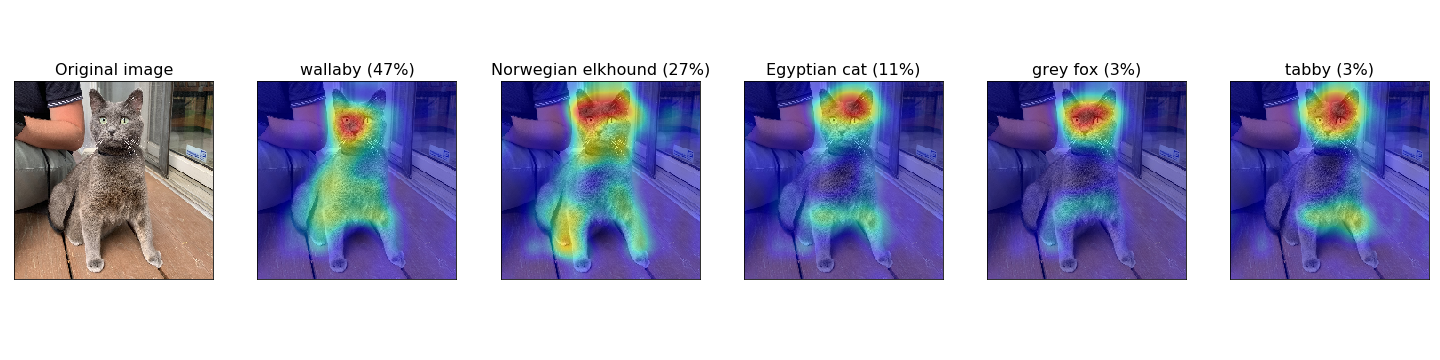
\includegraphics[width=6in]{csci-8110/hw-2/images/jeb_output.png}
    \caption{Jeb, the... wallaby?}
    \label{fig:jeb}
\end{figure}


\subsection{Model Observations}
\par Given that the Keras Vis library makes implementing Grad-CAM so straightforward, it was easy to understand, by inputting different images, how the model isolates features to determine what objects an image contains.
In the case of Jeb, the model does not correctly identify him as a cat.
For Oscar the dog, the model is \textit{much} more reliable:

\begin{figure}[H]
    \centering
    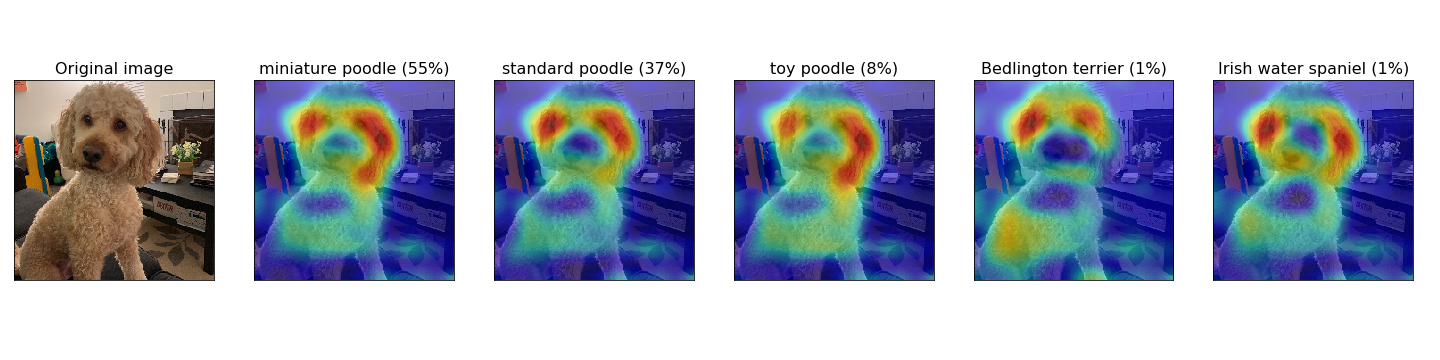
\includegraphics[width=6in]{csci-8110/hw-2/images/oscar_output.png}
    \caption{Oscar, the dog}
    \label{fig:oscar}
\end{figure}

\par For stock images, the model is extremely reliable:

\begin{figure}[H]
    \centering
    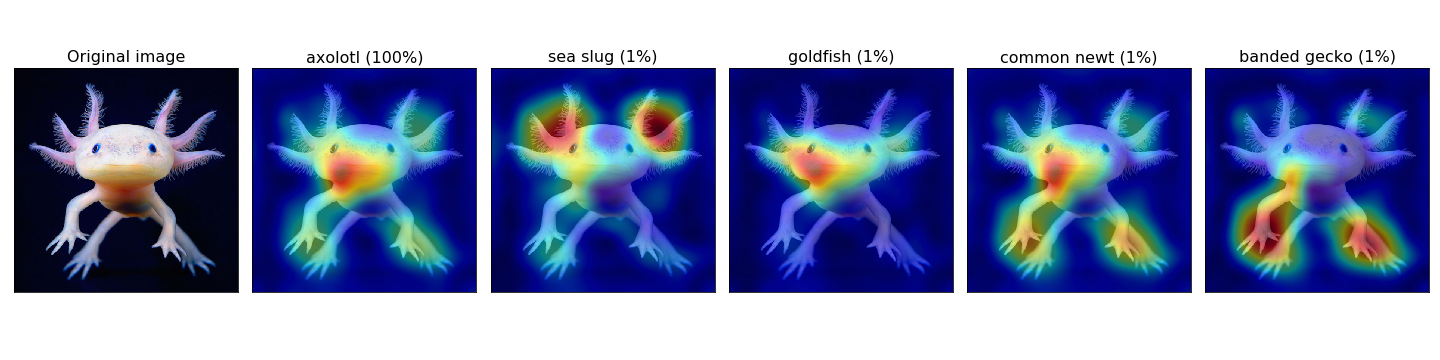
\includegraphics[width=6in]{csci-8110/hw-2/images/axolotl_output.png}
    \caption{An axolotl}
    \label{fig:axolotl}
\end{figure}

\par With the Grad-CAM heatmaps, being able to see the features that each category is "looking" at, is useful for identifying which attributes that the VGG16 model is using to identify an image, given a category.
This is even useful in situations, like with Jeb, where the model has room for refinement.

\par Ideally, the \lstinline{tf-keras-vis} library would have more room for experimentation, or this assignment would have been started with more time to fully implement a Grad-CAM implementation.
In either case, more could be done to visualize the impact of selected layers on the final heatmap.
All said, though, being able to understand the process that models use to identify images is a useful exercise.

\section{Conclusions}
One of the interesting traits of the CAM methods used in this project is that, as a visualization tool, the effectiveness of methods is predicated heavily on a well-trained model.
In practice, this meant that stock images of, say, a goldfish were easily recognizable by the model, where personal photos of a cat were misinterpreted.
Since the results of CAM mapping are tied so closely to that model, and since the process of training models currently feels somewhat out of view, it bears noting that an area of interest for future work might be around training and implementing more training for datasets. It was difficult to resist the urge to try and implement a more robust model for, say, a family member's pet. 
The possibility of doing that kind of work later in this course (or in future academic work) is attractive in that it would provide further opportunities to build an understanding of how neural networks can be supplied with better information on which to make inferences about data.

\par As it stands, though, this project was useful in terms of helping to develop a better understanding of how CNNs can be applied to explain the criteria upon which a trained model perceives input data to be one category (over another).
Being able to use provided Keras tools to implement this made for a somewhat easy assignment; this was so much the case that it felt somewhat uncomfortable writing only a few lines of code for submission.
The foundation provided by Assignment 1 and this assignment should be adequate to move on to more complex topics like training models to data or doing more robust image recognition.

\begin{appendices}

\newpage
\section{Model Output Listing} \label{modelouts}
\begin{figure}[H]
    \centering
    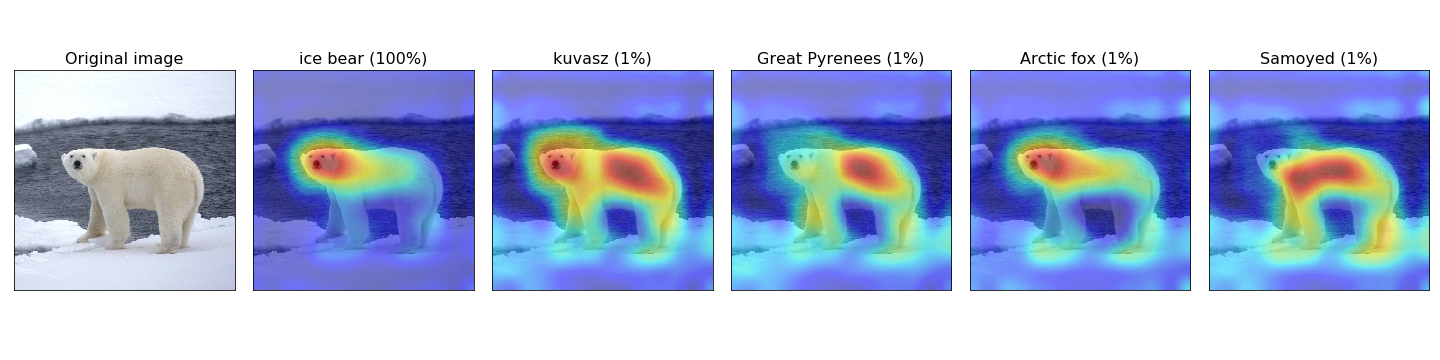
\includegraphics[width=6in]{csci-8110/hw-2/images/bear_output.png}
    \caption{A polar bear}
    \label{fig:bear}
\end{figure}
\begin{figure}[H]
    \centering
    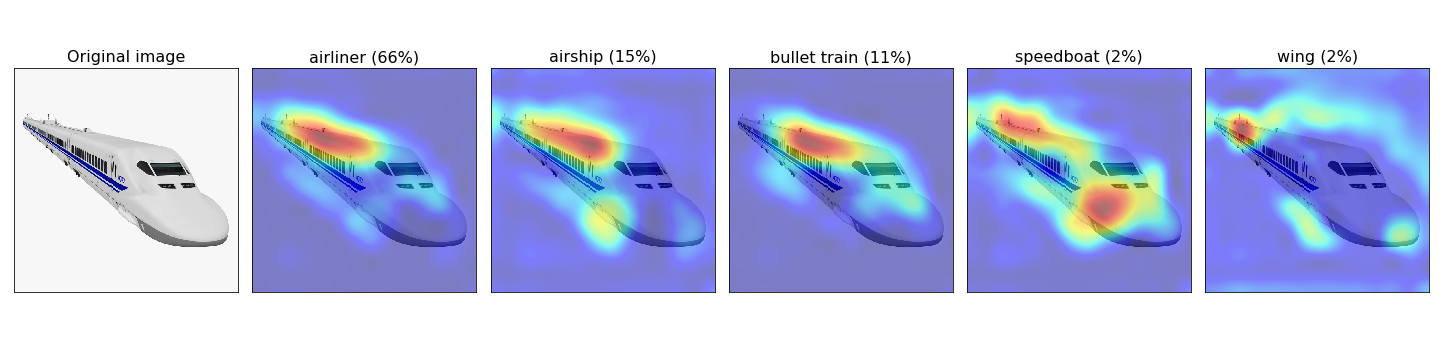
\includegraphics[width=6in]{csci-8110/hw-2/images/bullet_train_output.png}
    \caption{A bullet train}
    \label{fig:train}
\end{figure}
\begin{figure}[H]
    \centering
    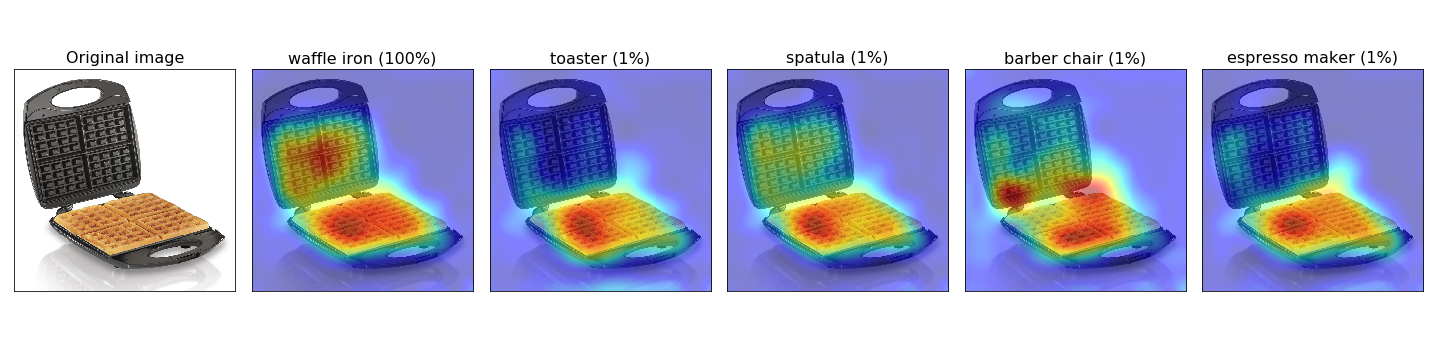
\includegraphics[width=6in]{csci-8110/hw-2/images/waffle_iron_output.png}
    \caption{A waffle iron}
    \label{fig:waffle}
\end{figure}
\newpage
\section{Complete Code Listing} \label{codelist}
\lstinputlisting[language=Python]{HW2_code.py}
\end{appendices}

\bibliographystyle{unsrt}
\bibliography{references}

\end{document}